\documentclass[border=10pt]{standalone}
\usepackage[svgnames]{xcolor}
\usepackage{amsmath}
\usepackage{pgfplots}
\pgfplotsset{compat=newest}
\usepackage[sfdefault]{FiraSans}
\usepackage{FiraMono}
\renewcommand*\familydefault{\sfdefault}
\begin{document}
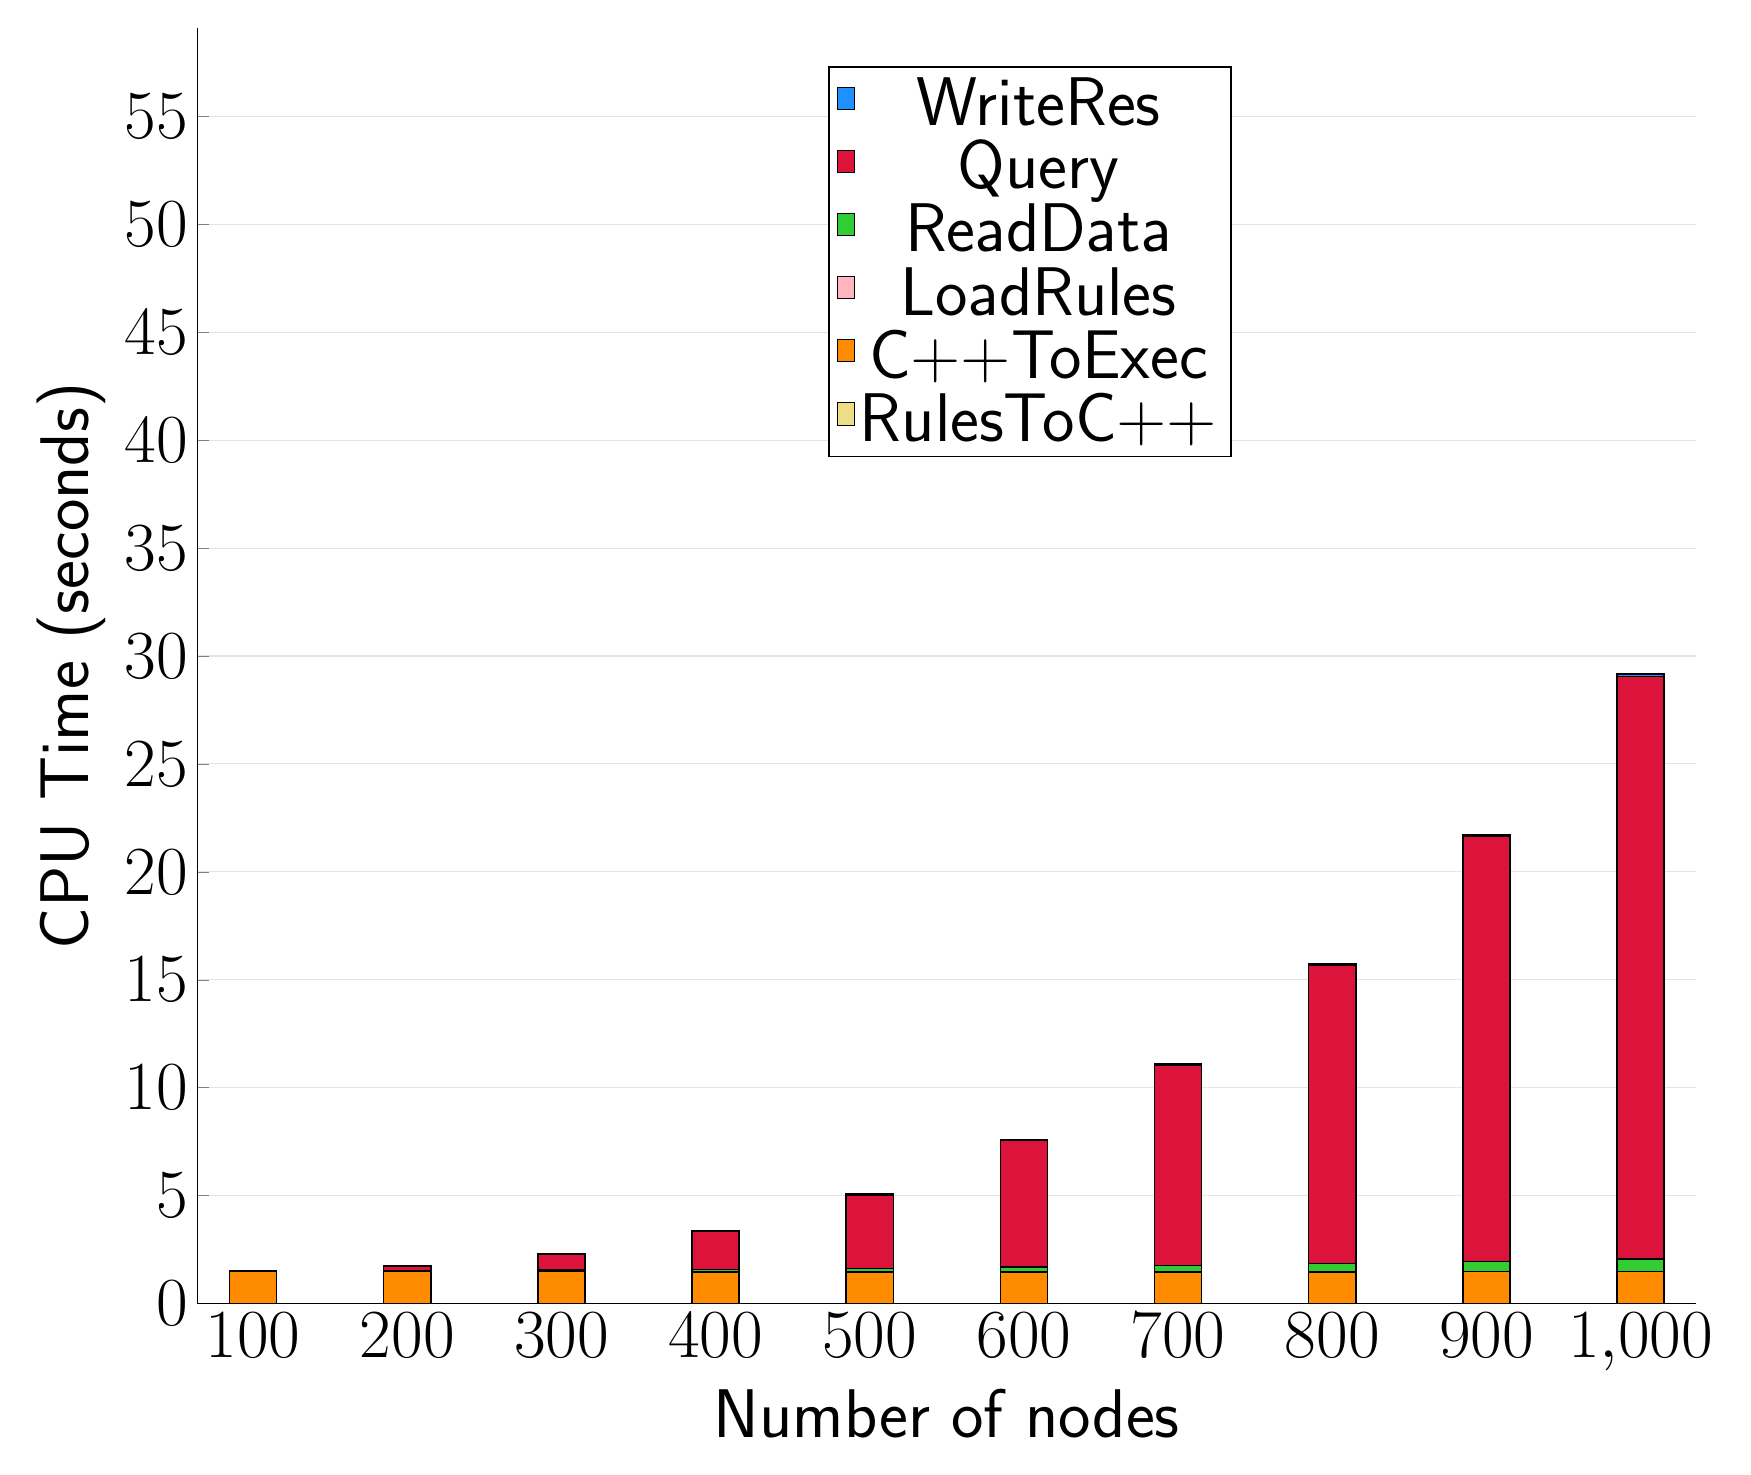
\begin{tikzpicture}
\begin{axis}[
   ybar stacked,
   width=1.7\textwidth,
   bar width=0.6cm,
   ymajorgrids, tick align=inside,
   major grid style={draw=gray!20},
   xtick=data,
   ymin=0, ymax=59.082040000000006,
   axis x line*=bottom,
   axis y line*=left,
   enlarge x limits=0.04,
   legend style={
       at={(0.69, 0.97)},
       anchor=north east,
       legend columns=1,
       font=\Huge,
   },
   ylabel={CPU Time (seconds)},
   xlabel={Number of nodes},
   label style={font=\Huge},
   tick label style={font=\Huge},
]
\addlegendimage{fill=DodgerBlue, draw=black, line width=0.2pt}
\addlegendentry{WriteRes}
\addlegendimage{fill=Crimson, draw=black, line width=0.2pt}
\addlegendentry{Query}
\addlegendimage{fill=LimeGreen, draw=black, line width=0.2pt}
\addlegendentry{ReadData}
\addlegendimage{fill=LightPink, draw=black, line width=0.2pt}
\addlegendentry{LoadRules}
\addlegendimage{fill=DarkOrange, draw=black, line width=0.2pt}
\addlegendentry{C++ToExec}
\addlegendimage{fill=LightGoldenrod, draw=black, line width=0.2pt}
\addlegendentry{RulesToC++}
\addplot +[fill=LightGoldenrod, draw=black, line width=0.55pt] coordinates {
(100, 0.006000000000000001)
(200, 0.0020000000000000005)
(300, 0.006000000000000001)
(400, 0.0020000000000000005)
(500, 0.0020000000000000005)
(600, 0.006000000000000001)
(700, 0.0020000000000000005)
(800, 0.0)
(900, 0.0020000000000000005)
(1000, 0.0020000000000000005)
};
\addplot +[fill=DarkOrange, draw=black, line width=0.55pt] coordinates {
(100, 1.472)
(200, 1.48)
(300, 1.4739999999999998)
(400, 1.474)
(500, 1.466)
(600, 1.47)
(700, 1.47)
(800, 1.476)
(900, 1.476)
(1000, 1.478)
};
\addplot +[fill=LightPink, draw=black, line width=0.55pt] coordinates {
(100, 0.000163)
(200, 0.0002028)
(300, 0.0001538)
(400, 0.0001672)
(500, 0.0001664)
(600, 0.00018559999999999998)
(700, 0.0001746)
(800, 0.00011920000000000001)
(900, 0.0001364)
(1000, 0.0001806)
};
\addplot +[fill=LimeGreen, draw=black, line width=0.55pt] coordinates {
(100, 0.014233)
(200, 0.0424916)
(300, 0.06924559999999999)
(400, 0.1118292)
(500, 0.1647)
(600, 0.2280462)
(700, 0.3022158)
(800, 0.380132)
(900, 0.47982440000000004)
(1000, 0.5931984)
};
\addplot +[fill=Crimson, draw=black, line width=0.55pt] coordinates {
(100, 0.0428654)
(200, 0.2289376)
(300, 0.7474725999999999)
(400, 1.7568139999999999)
(500, 3.4065500000000006)
(600, 5.860647999999999)
(700, 9.2762)
(800, 13.80716)
(900, 19.6714)
(1000, 26.983659999999997)
};
\addplot +[fill=DodgerBlue, draw=black, line width=0.55pt] coordinates {
(100, 0.0014314)
(200, 0.004534999999999999)
(300, 0.009944999999999999)
(400, 0.017435799999999998)
(500, 0.0270044)
(600, 0.038553000000000004)
(700, 0.052592799999999995)
(800, 0.0686184)
(900, 0.086324)
(1000, 0.1069372)
};
\end{axis}
\end{tikzpicture}

\end{document}
